Continuing from the previous task, the same tools listed before are used for the
continuation, that is finding and exploiting a buffer overflow on the
expensive\_calculator\_x86.

\section{Investigation}

After finding the valid key, we can identify sources of inputs. Let's test that
one for a buffer overflow vulnerability.

\begin{figure}[H]
  \centering
  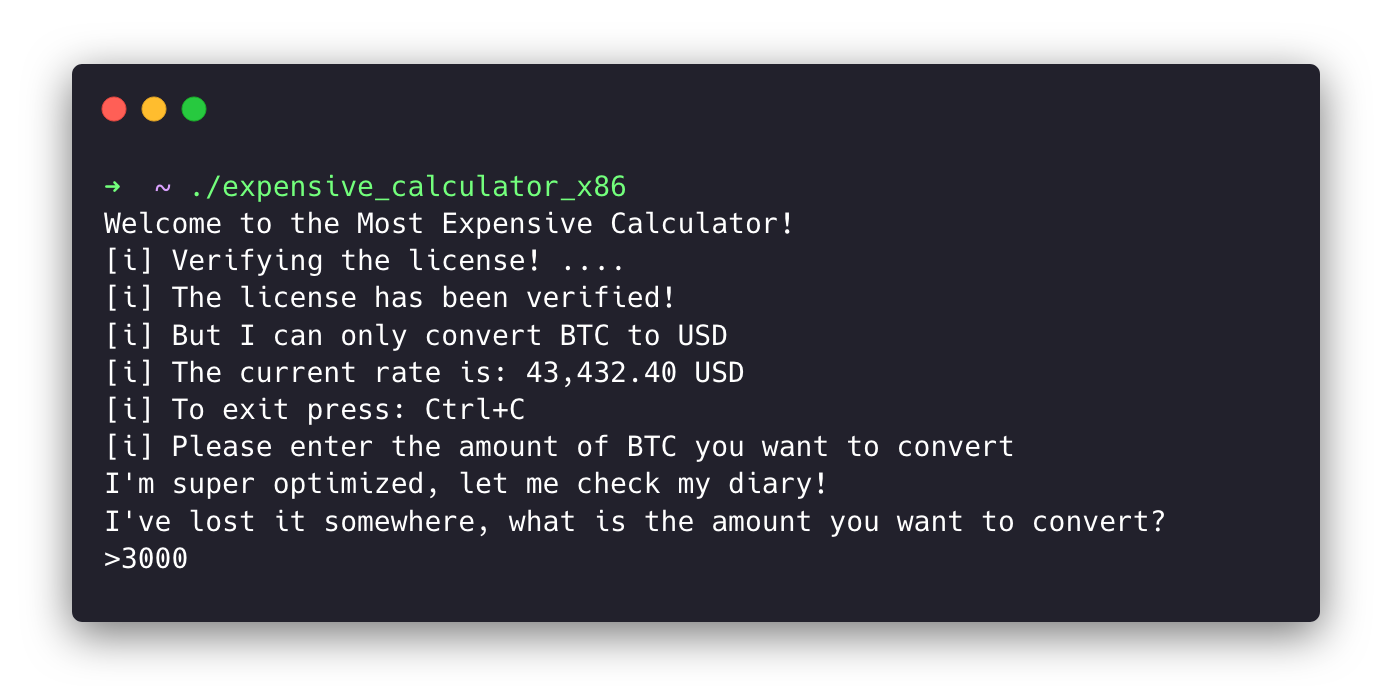
\includegraphics[width=0.8\textwidth]{figures/source-input}
  \caption{Sources of Inputs}
  \label{f:source-input}
\end{figure}

Let's investigate how that value interacts with the program in memory as it is
used somewhere for more processing. Digging in the decompiled output, the amount
conversion logic occurs in the calculator function.

\begin{figure}[H]
  \centering
  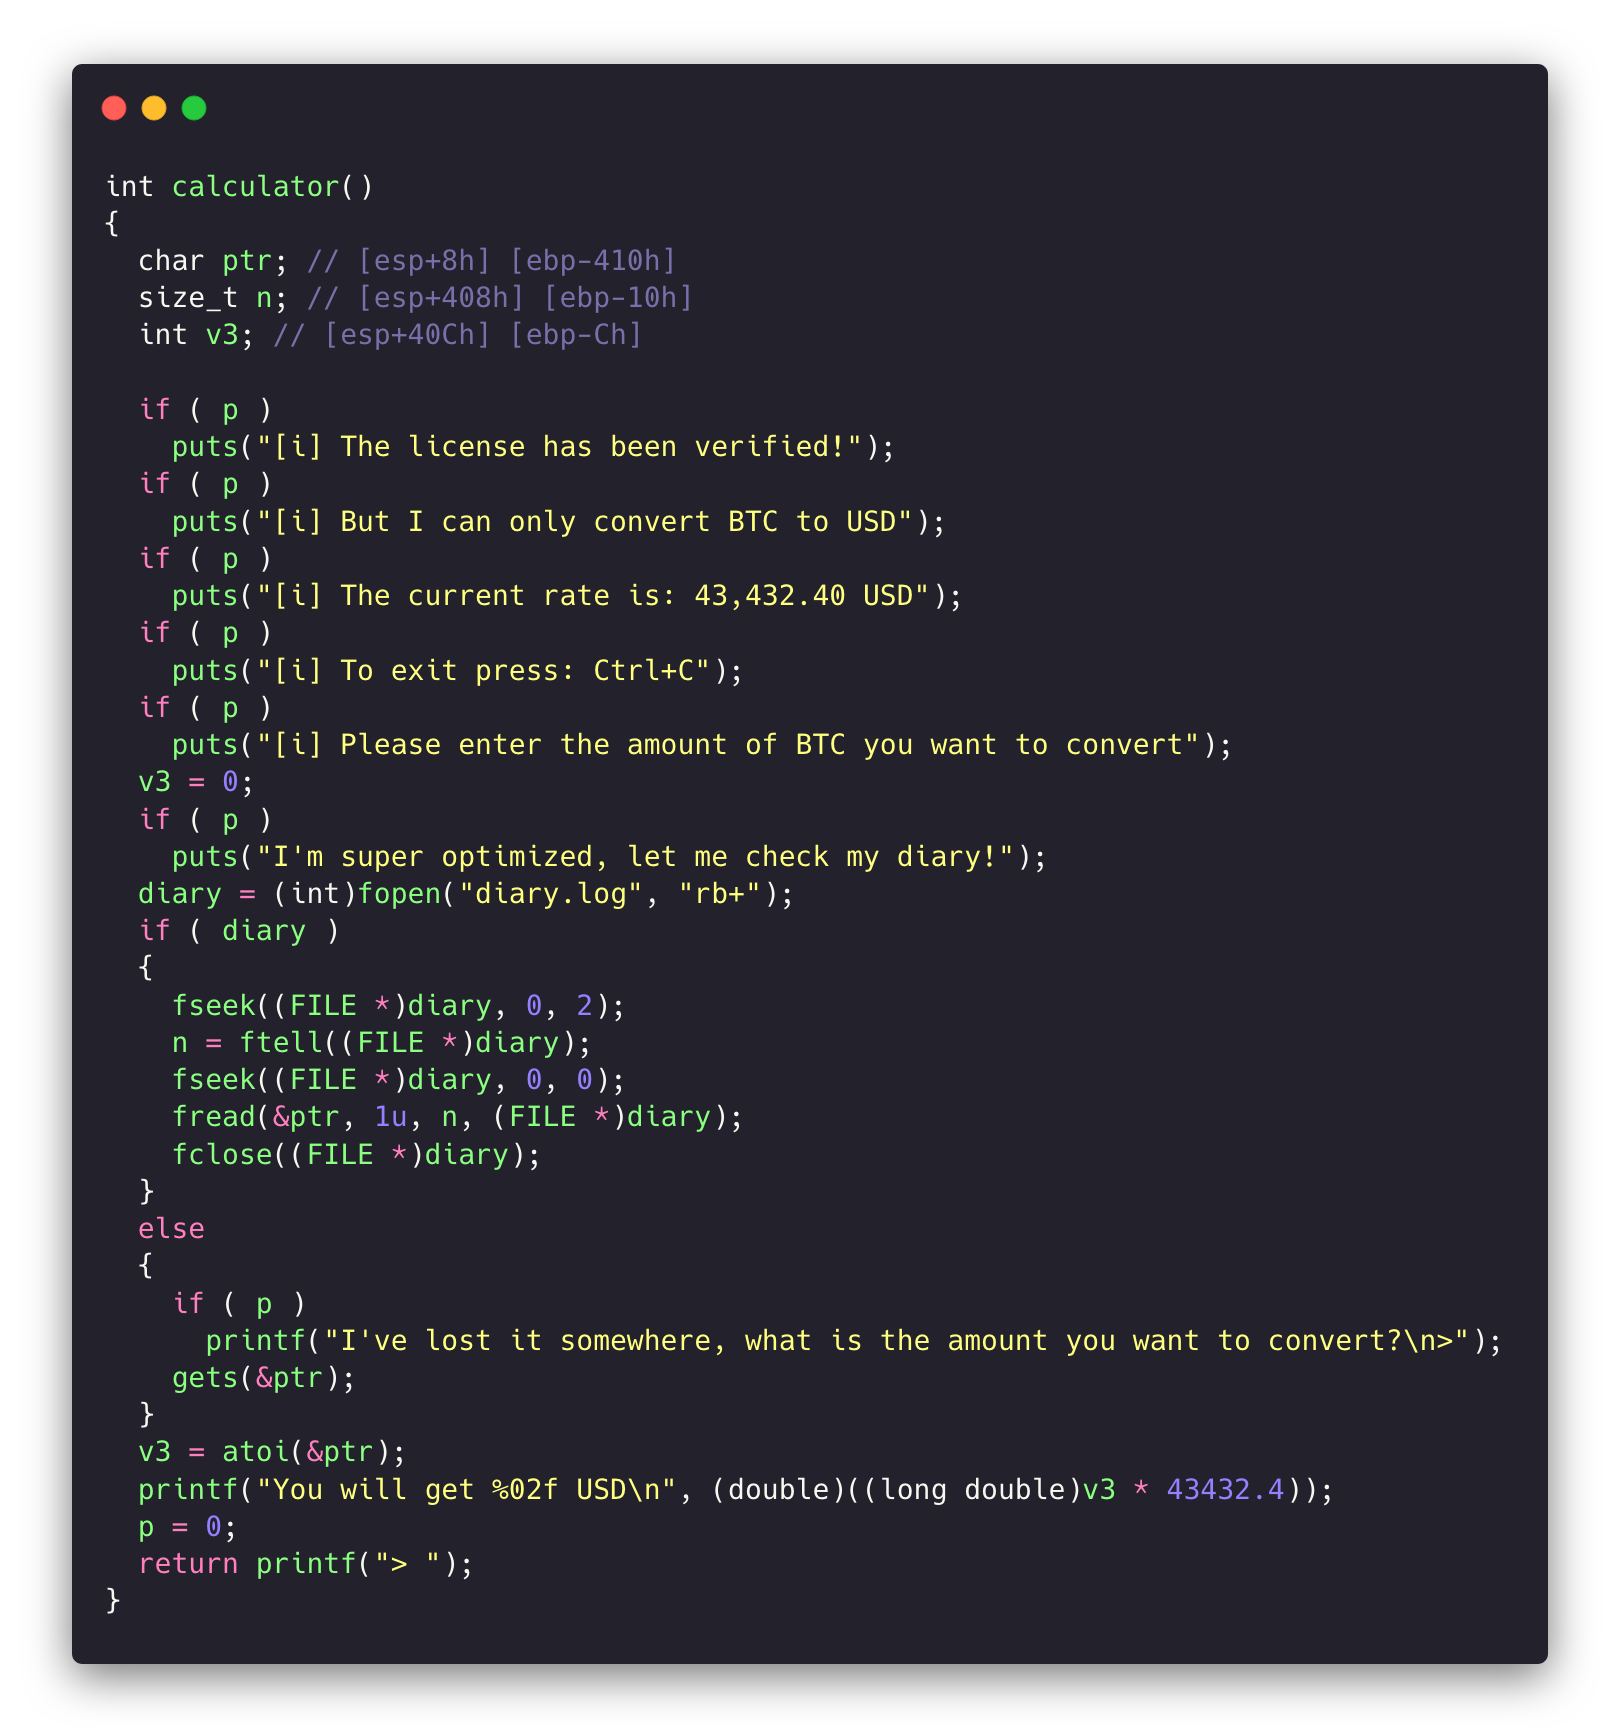
\includegraphics[width=0.6\textwidth]{figures/calculator}
  \caption{calculator}
  \label{f:calculator}
\end{figure}

We can note that the string 'what is the amount you want to convert?
\textbackslash n>' is the last print before asking for user input. Here the
executable uses gets, which has no defences against buffer overflow
vulnerabilities.
First of all we need to enable core dumps on linux. Then we can run GDB.

\begin{figure}[H] \centering
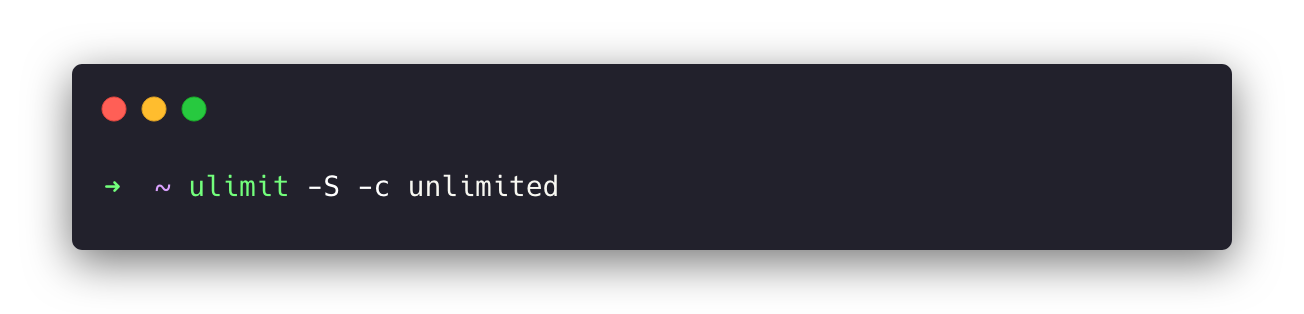
\includegraphics[width=1\textwidth]{figures/enable-core-dumps}
\caption{enable-core-dumps} \label{f:enable-core-dumps} \end{figure}

Using trial and error to find the number of characters needed to overflow, the
buffer is 1036 characters. Writing 1037 will cause the program to crash.

\begin{figure}[H]
  \centering
  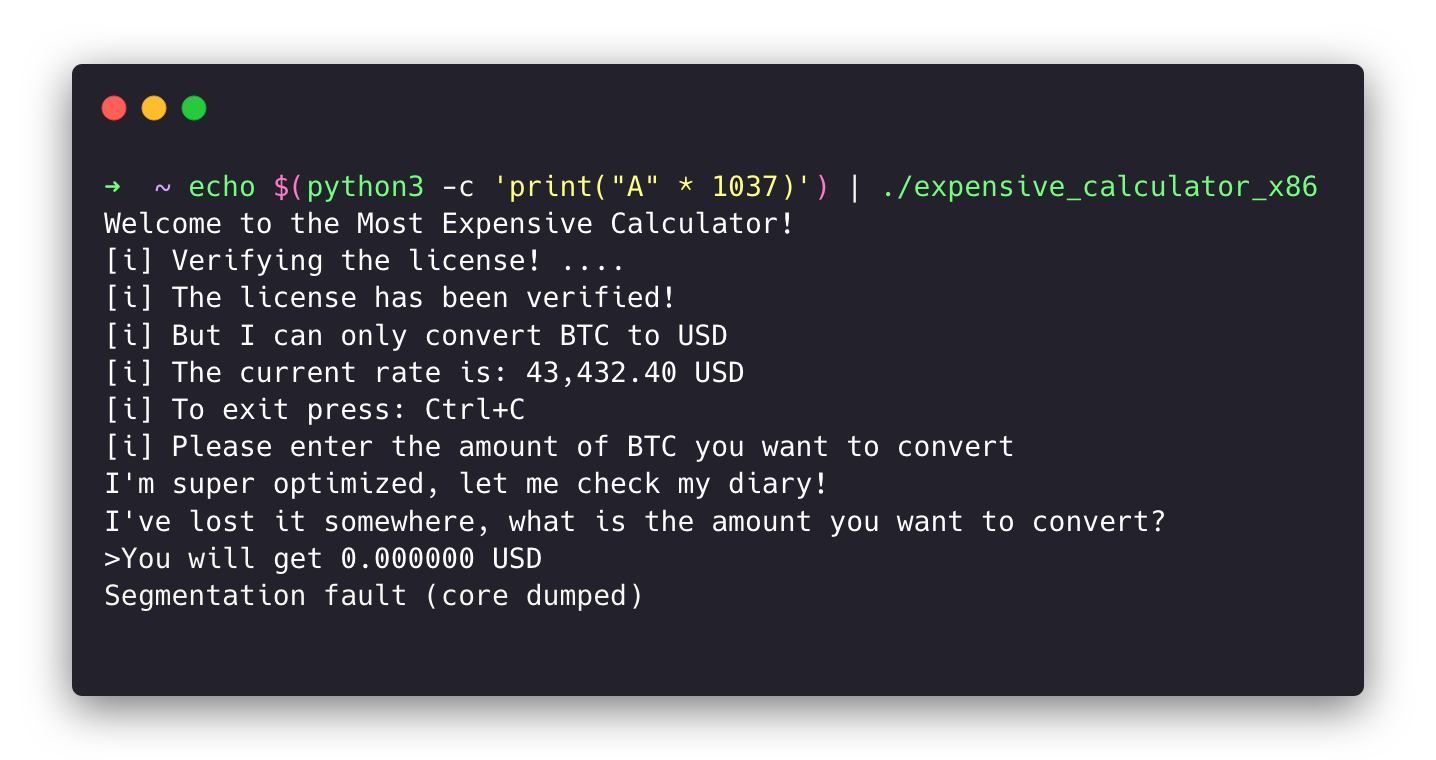
\includegraphics[width=0.8\textwidth]{figures/echo-python}
  \caption{Buffer 1037}
  \label{f:echo-python}
\end{figure}

The core is dumped, so let's have a look at it in GDB as we can triage this
crash.


\begin{figure}[H]
  \centering
  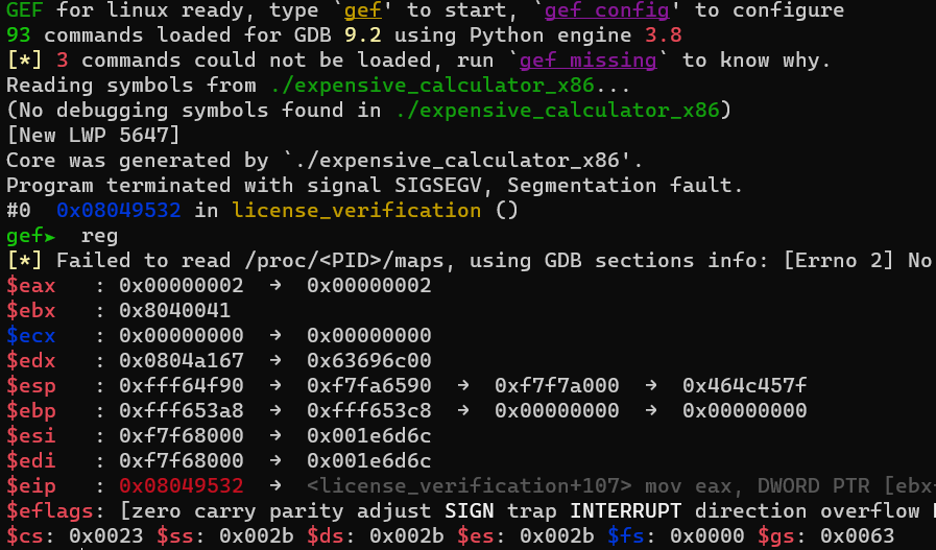
\includegraphics[width=0.7\textwidth]{figures/gdb1}
  \caption{Ebx register}
  \label{f:gdb1}
\end{figure}

Looking at the ebx register, 1 byte was overflown 0x41, which is A in ASCII\@.
Let's try to overwrite until the eip register. Replace 1037 with 1048, and we
notice in the new crash we have overwritten up to the instruction pointer (eip).

\begin{figure}[H]
  \centering
  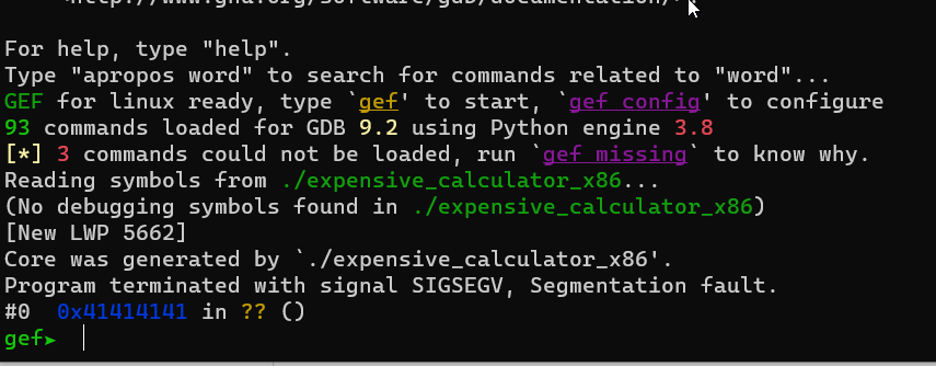
\includegraphics[width=0.7\textwidth]{figures/gdb2}
  \caption{Eip}
  \label{f:gdb2}
\end{figure}

We have control of the instruction pointer. But since this is a modern operating
system, and there are various mitigations at play such as Address space layout
randomization (ASLR), we cannot just write shellcode to memory and execute it.
What we can use here is Return Oriented Programming to get a shell on this.
These are the steps we will take:

\begin{enumerate}
  \item Leak address of \_\_libc\_start\_main
  \item Use the leaked address to calculate where libc is loaded by the
  executable
  \item Find system address in memory
  \item Find "/bin/sh" string in libc shared library in memory
  \item Arrange an ROP chain to execute the system with ``/bin/sh'' to get
  a shell.
\end{enumerate}

To leak the address of \_\_libc\_start\_main, we can redirect execution to
puts@plt and pass the Global Offset Table entry address for \_\_libc\_start\_main.
The following scripts utilise pwntools to achieve this.

\begin{figure}[H]
  \centering
  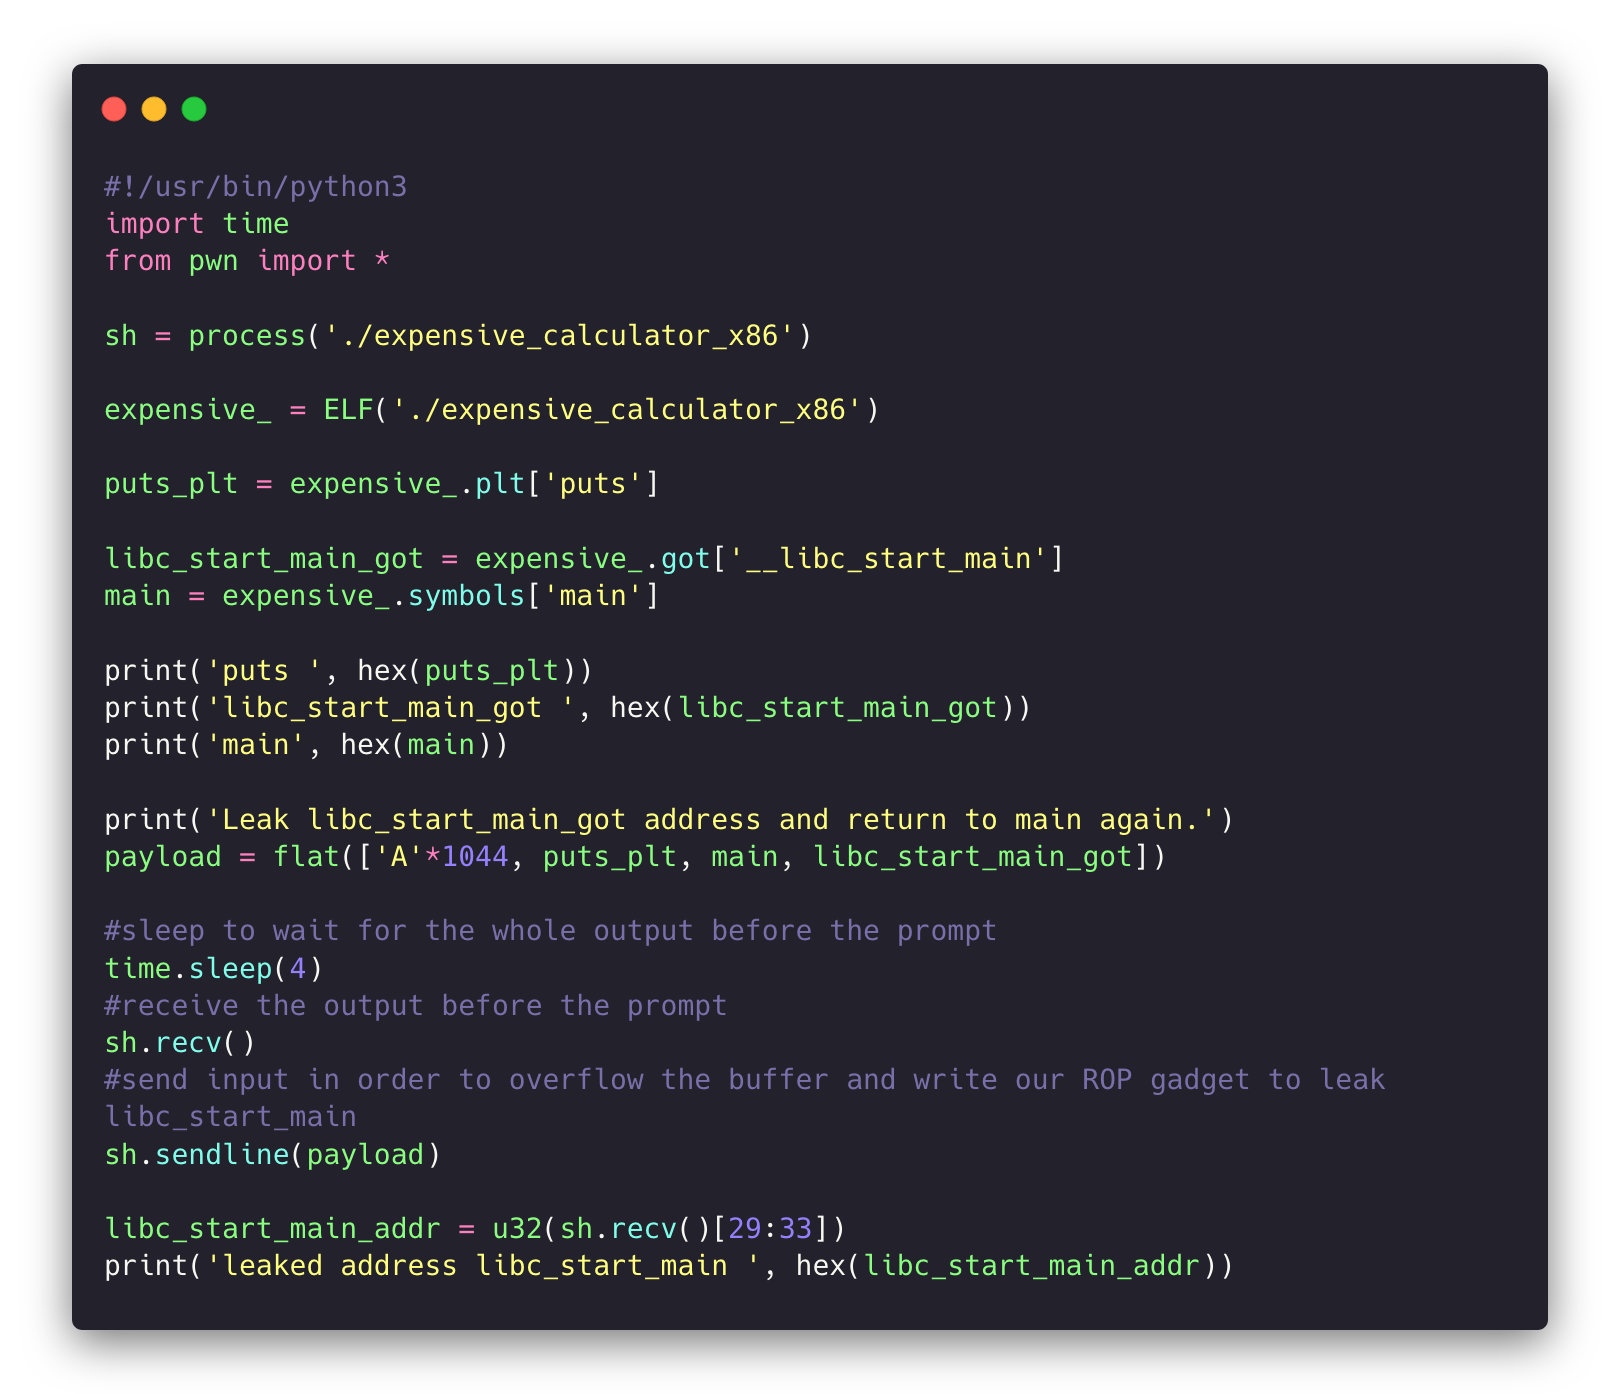
\includegraphics[width=0.8\textwidth]{figures/pwntools}
  \caption{CTF library pwntools}
  \label{f:pwntools}
\end{figure}

We import pwntools first using the statement "from pwn import *". The payload
variable is sent to the executable and overwrites the entire buffer up to eip
here, we place puts@plt address and what follows is the return address(here we
want to get back to main). The last is the GOT entry for libc\_start\_main. We
have to sleep to give the application to load until it asks us for input we send
(It sleeps for 4 seconds). We receive all the output before the prompt we send
our payload. After sending it, the magic happens, and we get back output within
it the leaked address. The reason why we read from 29 is that there is data
before that is printed, then our leaked address follows, and it is a 32-bit
address, so four bytes. Once we have the leaked address, we can calculate the
correct addresses of the system and the binsh string in memory. To do this, we
first get the base address for libc. Let us see which libc the executable loads
and its absolute path to get the symbol offsets for \_\_libc\_start\_main.
Running ldd on it, we get the following.

\begin{figure}[H]
  \centering
  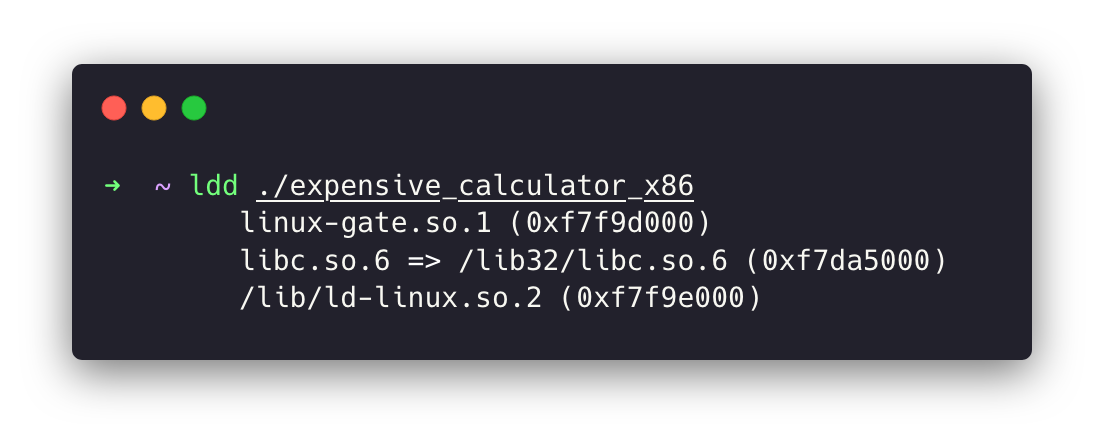
\includegraphics[width=0.8\textwidth]{figures/ldd}
  \caption{Libc executable with ldd}
  \label{f:ldd}
\end{figure}

We load this using pwntools ELF and get those symbols for \_\_libc\_start\_main
and system. Below the code that can run in the terminal.

\begin{figure}[H]
  \centering
  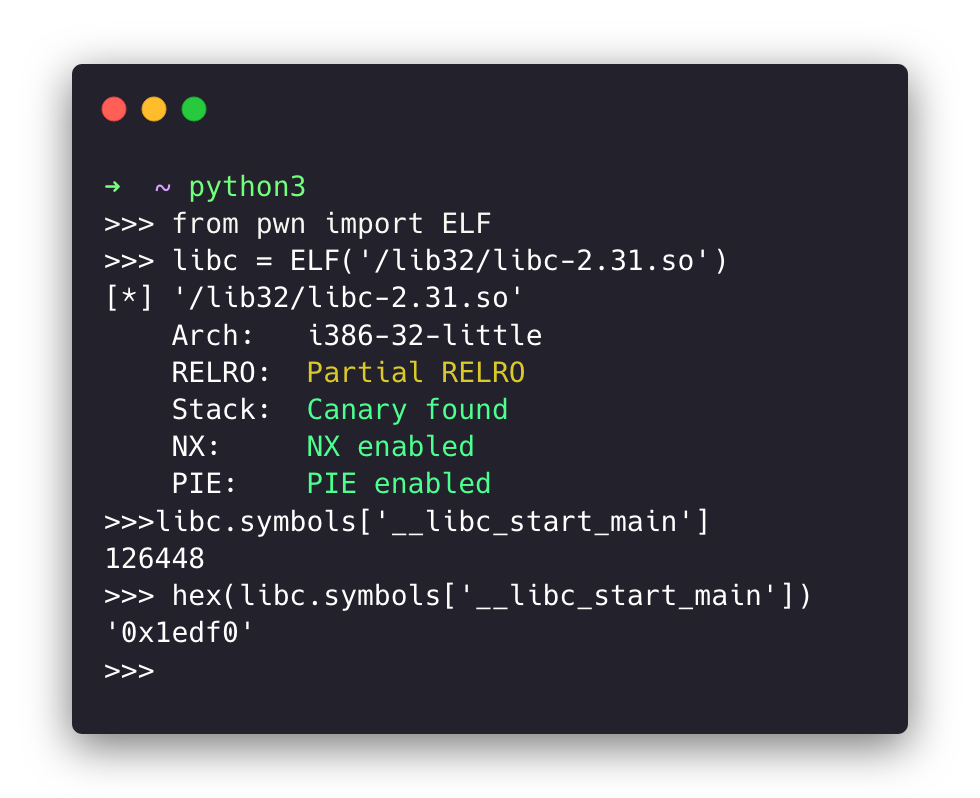
\includegraphics[width=0.6\textwidth]{figures/load-elf}
  \caption{ELF}
  \label{f:load-elf}
\end{figure}

To get the address for binsh, we use the following command to see the offset in
the libc-2.31.so library on disk.

\begin{figure}[H]
  \centering
  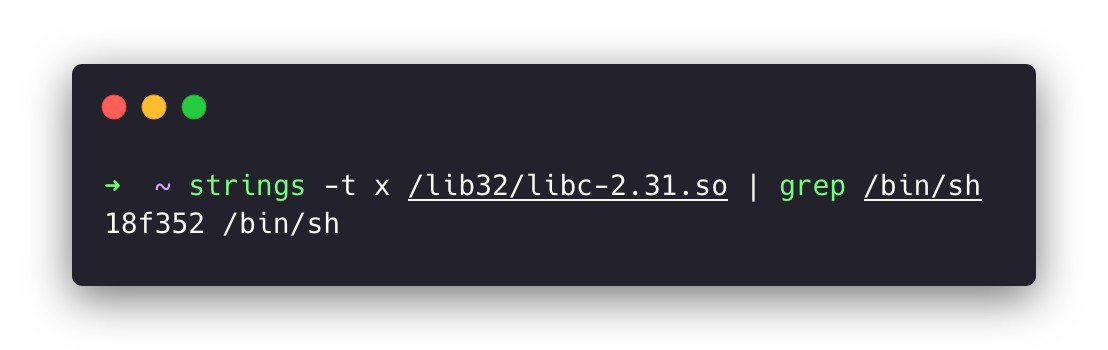
\includegraphics[width=0.6\textwidth]{figures/strings-t}
  \caption{Strings offset libc}
  \label{f:strings-t}
\end{figure}

We add the missing parts to the pwntool exploit base we previously wrote,
including libc base, system address and binsh address.

\begin{figure}[H]
  \centering
  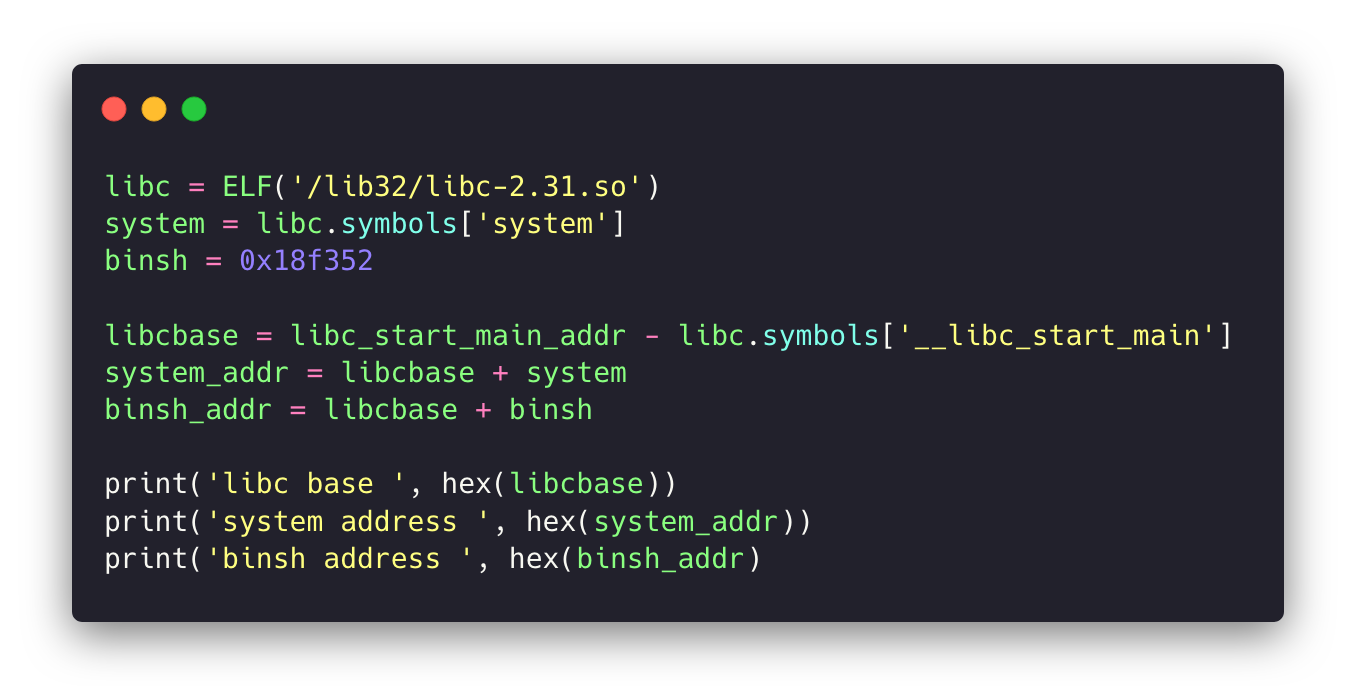
\includegraphics[width=0.8\textwidth]{figures/addresses}
  \caption{Addresses}
  \label{f:addresses}
\end{figure}

Then we also arrange our payload and send it again for us to get a shell.

\begin{figure}[H]
  \centering
  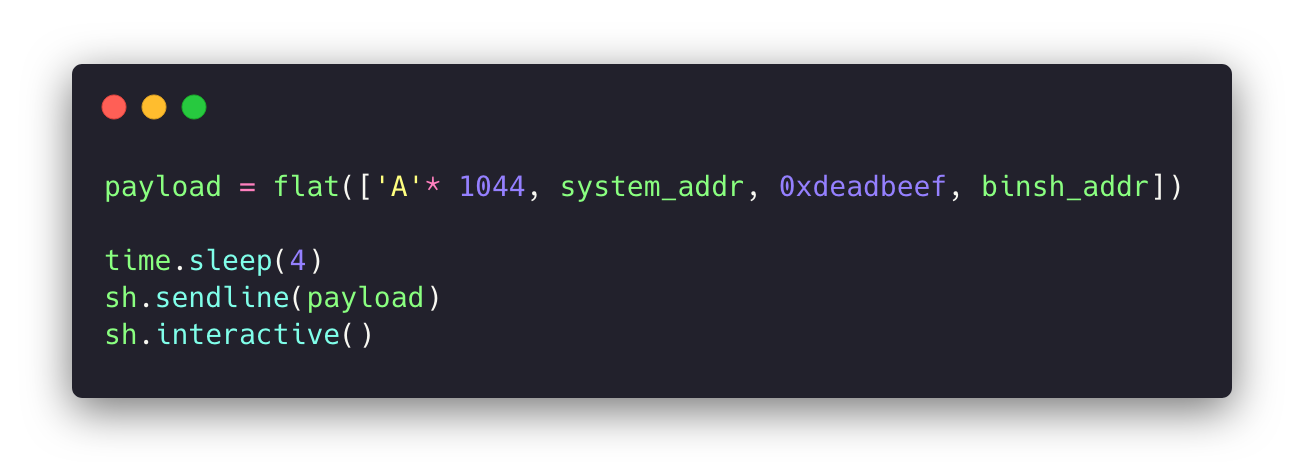
\includegraphics[width=0.8\textwidth]{figures/payload}
  \caption{Payload}
  \label{f:payload}
\end{figure}

We sleep, since we are back in main, and it waits for 4 seconds to get to the
prompt part. We overflow the buffer up to before eip we place the address for
system which is the actual location for system in memory. The next is not
required since returning is not needed, so the system will take the calculated
address parameter for where binsh is located in memory.

Running the exploit will finally give us a shell.

\begin{figure}[H]
  \centering
  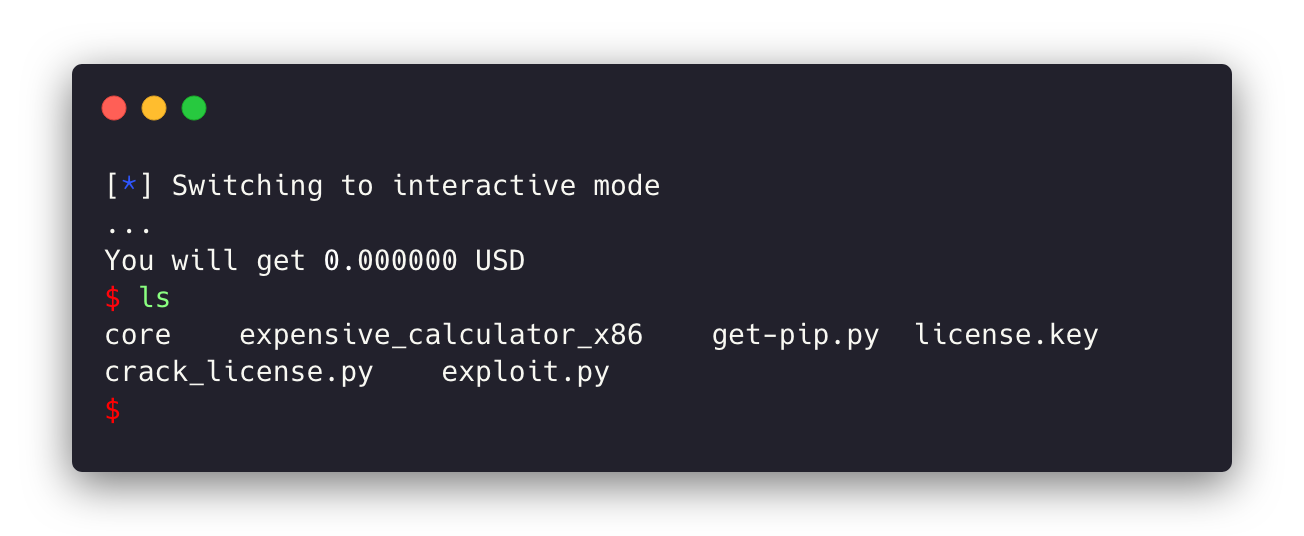
\includegraphics[width=0.8\textwidth]{figures/end}
  \caption{Shell}
  \label{f:end}
\end{figure}

The following is the whole script in python that can be used to succesfully
exploit the application through buffer overflow.

\begin{figure}[H]
  \centering
  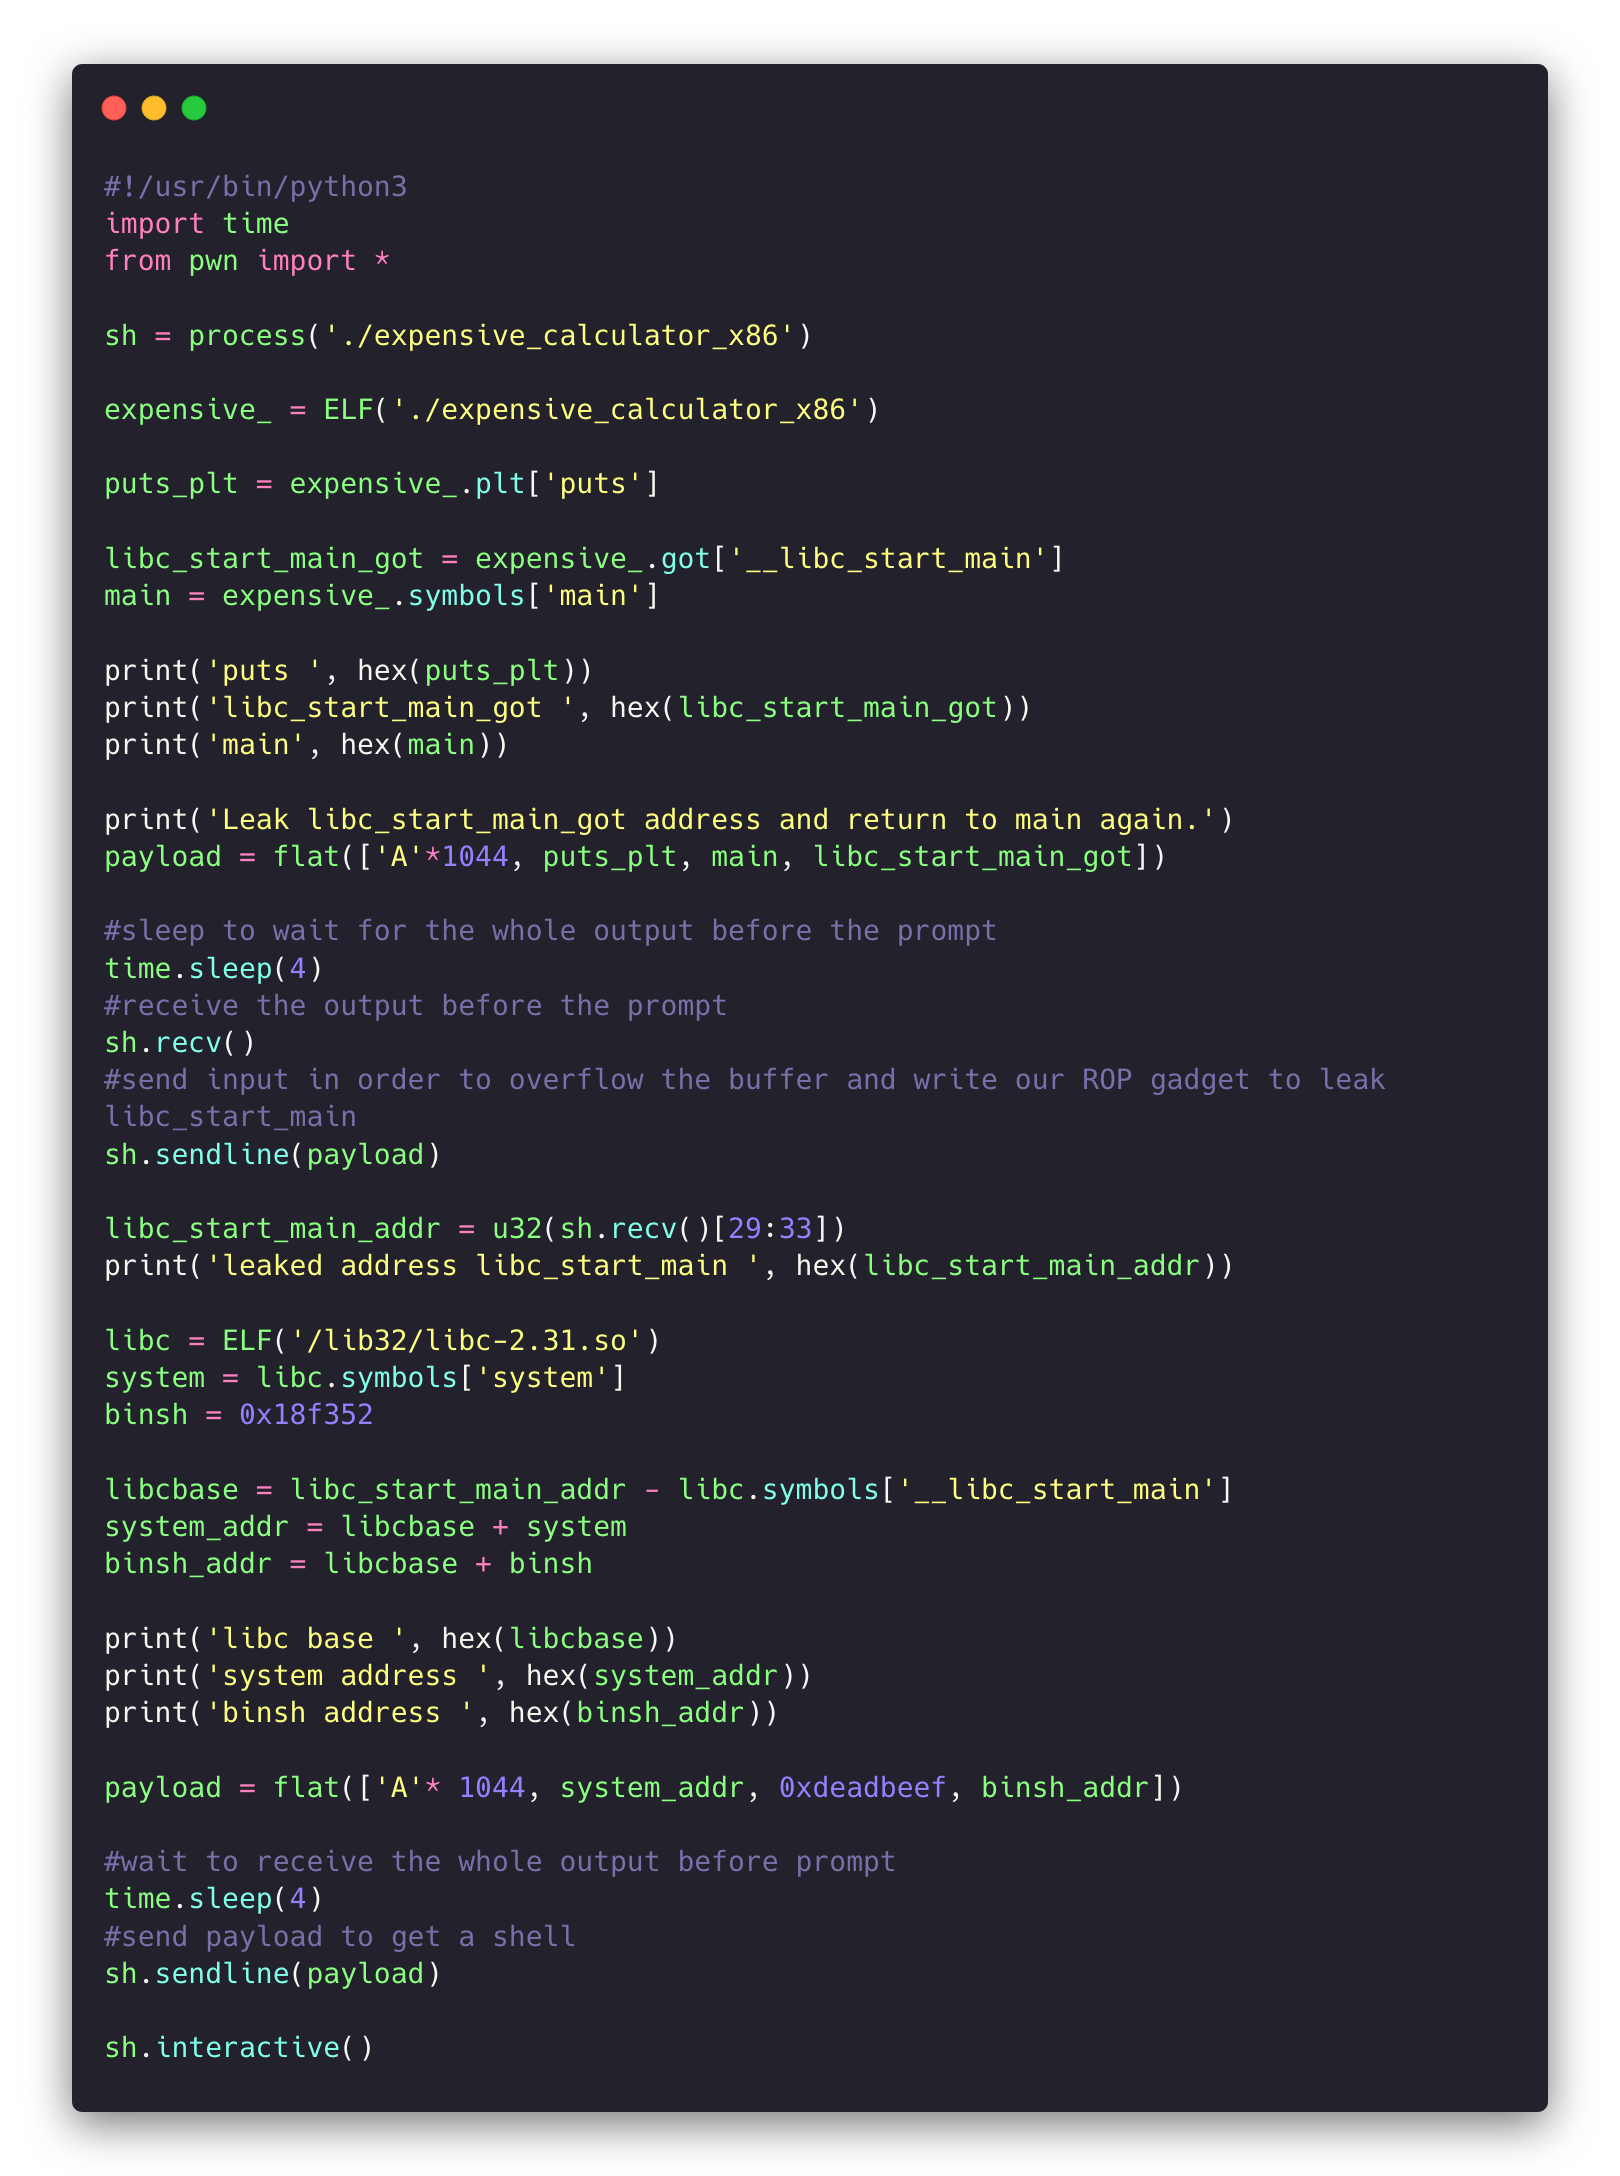
\includegraphics[width=0.75\textwidth]{figures/pwntools-full}
  \caption{Full exploit}
  \label{f:pwntools-full}
\end{figure}

\section{Conclusion}
\label{s:conclusion-lab-6}
This is the last lab of the module and it has been the most challenging one.
Buffer overflow is a vulnerability that can cause a lot of damage and still
troubles engineers in the world. The lab has been a great learning experience
but needed a lot of research and time to get it done.
